\begin{center}
  \Large
  \textbf{BIOGRAFI PENULIS}
\end{center}

\addcontentsline{toc}{chapter}{BIOGRAFI PENULIS}

\vspace{2ex}

\begin{wrapfigure}{L}{0.3\textwidth}
  \centering
  \vspace{-3ex}
  % Ubah file gambar berikut dengan file foto dari mahasiswa
  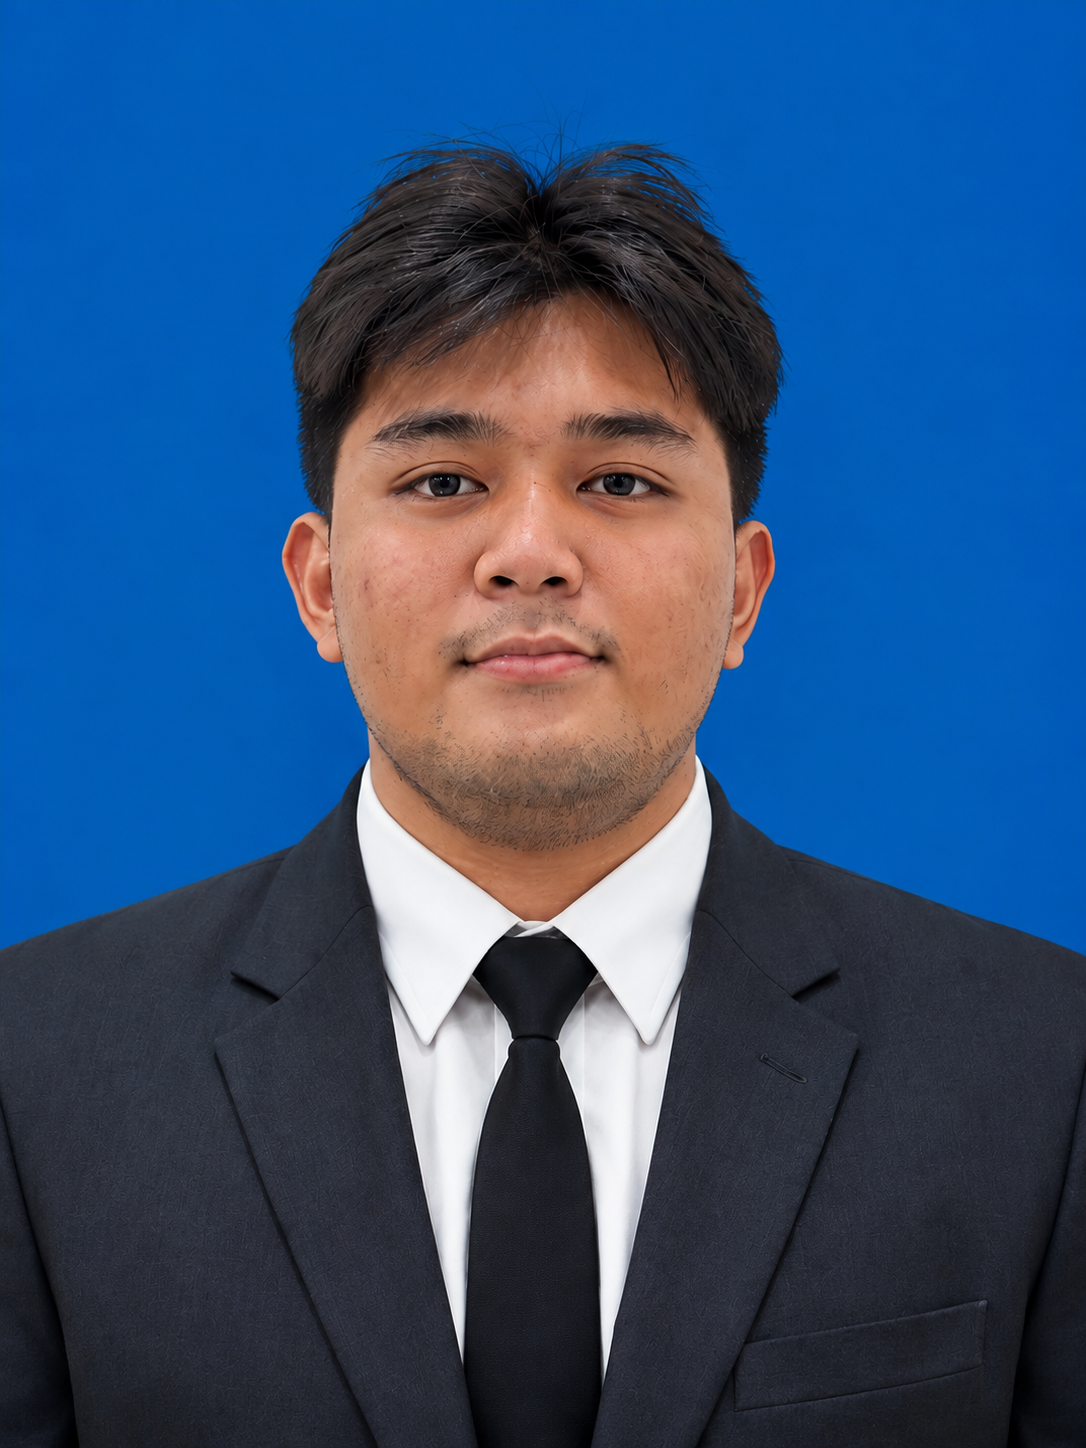
\includegraphics[width=0.3\textwidth]{gambar/biografi.png}
  \vspace{-4ex}
\end{wrapfigure}

% Ubah kalimat berikut dengan biografi dari mahasiswa
\noindent Yoel Yhokhanan Sianipar, penulis buku tugas akhir 
berjudul \textit{"Sistem Pengendalian Tekanan Pompa Air Berbasis Inverter dengan Neural Network"}, 
lahir di Medan pada tanggal 29 September 2004 dan merupakan anak pertama dari tiga bersaudara. 
Penulis telah menempuh pendidikan formal di SD Latihan HKBP Pearaja Tarutung, 
SMPK Immanuel Batam, dan SMAN 1 Batam. Setelah lulus dari sekolah 
menengah atas pada tahun 2022, penulis melanjutkan studi di Departemen Teknik Elektro, Fakultas 
Teknologi Elektro dan Informatika Cerdas (FTEIC), Institut Teknologi Sepuluh Nopember 
(ITS) melalui jalur UTBK-SBMPTN dengan NRP 5022221081. Selama masa perkuliahan, penulis aktif berorganisasi dan 
mengembangkan diri, khususnya di bidang energi baru dan terbarukan (EBT). 
Penulis bergabung sebagai anggota di \textit{Society of Renewable Energy} (SRE) ITS. 
Ketertarikan yang mendalam terhadap teknologi hijau tersebut membawa penulis 
untuk berkontribusi lebih jauh di Antasena ITS Team sebagai \textit{Electronics \& Powertrain Engineer}. 
Penulis memiliki ketertarikan akademis dan profesional yang sangat besar pada integrasi sistem 
tenaga listrik dan elektronika, yang diimplementasikan secara nyata melalui riset tugas akhir ini.
